
\documentclass[12pt]{article}


\usepackage{amssymb}
\usepackage{amsmath,amsthm, mathtools}
\usepackage{graphics, color}

\usepackage{graphicx}
\usepackage{epsfig}
\usepackage{makeidx}
\usepackage{kotex}
\usepackage{fullpage}
%\makeindex
%https://www.overleaf.com/project/62dae1f79296e5799bd3cf6d

\hbadness=10000 \tolerance=10000 \hyphenation{en-vi-ron-ment
in-ven-tory e-num-er-ate char-ac-ter-is-tic}



\usepackage[round]{natbib}
%\bibliographystyle{apalike2}
% \bibliographystyle{jmr}


\newcommand{\biblist}{\begin{list}{}
{\listparindent 0.0cm \leftmargin 0.50cm \itemindent -0.50 cm
\labelwidth 0 cm \labelsep 0.50 cm
\usecounter{list}}\clubpenalty4000\widowpenalty4000}
\newcommand{\ebiblist}{\end{list}}

\newcounter{list}


%\usepackage{setspace}
\usepackage{comment}
\usepackage{latexsym}
\usepackage{amsmath, amssymb, amsfonts, amsthm, bbm}
\usepackage{graphicx}
\usepackage{mathrsfs}

\newcommand{\bb}[1]{\mathbb{#1}}
\renewcommand{\bf}[1]{\boldsymbol{\mathbf{#1}}}
\renewcommand{\cal}[1]{\mathcal{#1}}
\renewcommand{\frak}[1]{\mathfrak{#1}}

\newcommand{\quation}[1]{\begin{equation*}#1\end{equation*}}
\newcommand{\lign}[1]{\begin{align*}#1\end{align*}}
\newcommand{\lignat}[2]{\begin{alignat*}{#1}#2\end{alignat*}}
\newcommand{\ather}[1]{\begin{gather*}#1\end{gather*}}
\newcommand{\ultline}[1]{\begin{multline*}#1\end{multline*}}
\newcommand{\ases}[1]{\begin{cases}#1\end{cases}}

\newcommand{\obar}[1]{\overline{#1}}
\newcommand{\ubar}[1]{\underline{#1}}

\newcommand{\set}[1]{\left\{#1\right\}} % {abc} % braces
\newcommand{\pa}[1]{\left(#1\right)} % (abc) % parentheses
\newcommand{\ang}[1]{\left<#1\right>} % <abc> % angle brackets
\newcommand{\bra}[1]{\left[#1\right]} % [abc] % brackets
\newcommand{\abs}[1]{\left|#1\right|} % |abc|
\newcommand{\norm}[1]{\left\|#1\right\|} %||abc||

\newcommand{\mat}[1]{\begin{matrix}#1\end{matrix}} % \mat{1 & 0 & 1 \\ 0 & 0 & 1 \\ 1 & 1 & 0}
\newcommand{\pmat}[1]{\pa{\mat{#1}}}
\newcommand{\bmat}[1]{\bra{\mat{#1}}} 

\newcommand{\sm}[1]{\begin{smallmatrix}#1\end{smallmatrix}}
\newcommand{\psm}[1]{\pa{\sm{#1}}}
\newcommand{\bsm}[1]{\bra{\sm{#1}}}

\newcommand{\tci}[2]{\set{\,#1 \mid{} #2\,}}
\newcommand{\pfrac}[2]{\pa{\frac{#1}{#2}}}
\newcommand{\der}[2]{\frac{\partial #1}{\partial #2}}
\newcommand{\pder}[2]{\pfrac{\partial #1}{\partial #2}}

\newcommand{\firstp}[2]{\ensuremath{\displaystyle
     \frac{\partial{#1}}{\partial{#2}}}} % \firstp{f}{x}
\newcommand{\secondp}[3]{\ensuremath{\displaystyle
     \frac{\partial^{2}{#1}}{\partial{#2}\,\partial{#3}^T}}} % \secondp{f}{x}{y}
\newcommand{\secondpscalar}[3]{\ensuremath{\displaystyle
     \frac{\partial^{2}{#1}}{\partial{#2}\,\partial{#3}}}} % \secondp{f}{x}{y}

%%%%%%%%%%%%%%%%%%%% OPERATORS %%%%%%%%%%%%%%%%%%%%
\DeclareMathOperator{\diag}{diag}
\DeclareMathOperator{\sgn}{sgn}
\DeclareMathOperator{\tr}{tr}
\DeclareMathOperator{\SE}{SE}
\DeclareMathOperator{\Var}{Var}
\DeclareMathOperator{\Cov}{Cov}
\DeclareMathOperator{\Corr}{Corr}
\DeclareMathOperator*{\argmax}{arg\,max}
\DeclareMathOperator*{\argmin}{arg\,min}

%%%%%%%%%%%%%%%%%%%% LETTERS %%%%%%%%%%%%%%%%%%%%
\newcommand{\N}{\mathbb{N}}
\newcommand{\Z}{\mathbb{Z}}
\newcommand{\Q}{\mathbb{Q}}
\newcommand{\R}{\mathbb{R}}

\newcommand{\iidsim}{\stackrel{i.i.d.}{\sim}}
\newcommand{\iid}{\stackrel{i.i.d.}{\sim}}

\newcommand{\st}{\text{ }s.t.\text{ }}

\newcommand{\dps}{\displaystyle}
\usepackage{multirow}
\usepackage{subfigure}
\usepackage{enumitem}

\newcommand{\rank}{\text{rank}}

\begin{document}

\title{Double GREG estimator}

\maketitle

\section{Problem setup}
\begin{itemize}
    \item Let \(A\) be a sample of size \(n\) selected from the population
\(U\) of size \(N\). Let $\pi_i$ be the first order inclusion probability of unit $i$ and $\pi_{ij}$ the second order inclusion probability of unit $i$ and $j$.
\item Let \(y\) denote a variable of interest and we try to estimate the population total \(t_y = \sum_{i \in U} y_i\). Let \(\bf x_{i}\) of size \(p\) be the auxiliary variables associated with \(y\). 
Assume that $\bf x_i$ is observed throughout the finite population while $y_i$ is observed only in the sample.
\item Suppose the following superpopulation model holds
\begin{equation}
    y_i = \bf x_i^T \bf \beta + \varepsilon_i, \quad \varepsilon_i \iid (0,\sigma^2), \quad i = 1, \cdots, N \label{lin}
\end{equation}
\item Indeed, the linear regression model can be extended to the general nonlinear model whose basis function can be (penalized) spline functions. \eqref{lin} can be replaced by
\begin{equation}
    y_i = \sum_{j = 0}^Mh_j(\bf x_i) \beta_j + \varepsilon_i, \quad \varepsilon_i \iid (0,\sigma^2), \quad i = 1, \cdots, N 
\end{equation}
where $h_j(\cdot)$ are the corresponding basis functions. In this article, for the sake of simplicity, we assume linear basis functions in \eqref{lin} only.
\item The working model \eqref{lin} motivates the GREG estimator defined by
\begin{equation}
    \hat t_y = \sum_{i \in U}\bf x_i^T \hat {\bf \beta} + \sum_{i \in A}\frac{1}{\pi_i}\pa{y_i - \bf x_i^T \hat {\bf \beta}} \label{GREG}
\end{equation}
where $\hat {\bf \beta}$ is defined by
$$
\hat {\bf \beta} = \pa{\sum_{i \in A} \frac{1}{\pi_i}\pa{\bf x_i - \bar {\bf x}}\pa{\bf x_i - \bar {\bf x}}^T}^{-1}\pa{\sum_{i \in A} \frac{1}{\pi_i}\pa{\bf x_i - \bar {\bf x}}y_i}
$$
\eqref{GREG} enjoys many desirable design properties including asymptotic equivalence to the difference estimator which is defined by replacing the estimated $\hat {\bf \beta}$ by the known $\bf \beta$ in \eqref{GREG}. The GREG estimator is also known to be design consistent, asymptotically design unbiased, and asymptotically normally distributed with finite variance. Furthermore, its design variance can consistently be estimated by the linearized variance estimator
\begin{equation}
    \hat V_p = \sum_{i,j \in A} \frac{\Delta_{ij}}{\pi_{ij}} \frac{y_i - \bf x_i \hat {\bf \beta}}{\pi_i}\frac{y_j - \bf x_j \hat {\bf \beta}}{\pi_j} \label{var}
\end{equation}
However, when the number of parameters $p$ grows as $n$ increases, the properties listed above no longer hold.
\end{itemize}

\section{Double GREG estimator}
\begin{itemize}
    \item Now, suppose that $p$ is allowed to increase as the sample size increases. In the high-dimension setup, the estimating errors of the regression coefficients $\hat {\bf \beta}$ are no longer negligible and the GREG estimator is no longer asymptotically equivalent to the difference estimator since
$$
\hat t_{y, GREG} - \hat t_{y, diff} = 
\pa{\sum_{i \in U} \bf x_i - \sum_{i \in A}\frac{1}{\pi_i} \bf x_i } \pa{\hat {\bf \beta} - \bf \beta} \neq o_p(n^{-1}) 
$$
Indeed, \cite{ta2020generalized} recently showed that 
the GREG estimator is asymptotically equivalent to the difference estimator only if $p / n \to 0$.
    \item Furthermore, unlike fixed $p$ where the bias ($O(n^{-1})$) of the GREG estimator is negligible compared to the standard error($O(n^{-1/2})$) \citep{cochran1977sampling}, the bias of the high dimensional GREG estimator can be significant. The simulation results show that such a tendency manifests itself even stronger when the sampling design is informative (in the next section). One possible way to remove bias is by applying the jackknife method to the GREG estimator, but it does not account for high dimensional variables.
    \item In this regard, we consider the sample split method. Let $A_1$ and $A_2$ be a random partition of $A$ (possibly of equal size). Let $\hat {\bf \beta}_1$ and $\hat {\bf \beta}_2$ be the generalized regression coefficients using $A_1$ and $A_2$ respectively. We propose the double GREG estimator defined as follows
    \begin{equation}
  \hat t_y = \sum_{i \in U}\bf x_i^T\tilde {\bf \beta}  + \sum_{i \in A_1} d_i \pa{y_i - \bf x_i^T \hat{\bf \beta}_2} + \sum_{i \in A_2} d_i \pa{y_i - \bf x_i^T \hat{\bf \beta}_1} \label{double}        
    \end{equation}
  where $\tilde {\bf \beta}$ is the weighted regression coefficient defined by
  \begin{equation}
        \tilde {\bf \beta} = \frac{\sum_{i \in A_2}d_i}{\sum_{i \in A}d_i} \hat{\bf \beta}_1 + \frac{\sum_{i \in A_1}d_i}{\sum_{i \in A}d_i} \hat{\bf \beta}_2 
  \end{equation}
  \item Because of the random split, the resulting double GREG estimator can suffer from large variance. In order to reduce the variance and improve efficiency, we take several random splits from a sample and take the average of all the samples.
  That is, for each of the random sample $A_1(1), \cdots, A_1(K)$ and $A_2(1), \cdots, A_2(K)$ the final ensemble estimator is defined as
  \begin{equation}
      \hat t_y = \frac{1}{K}\sum_{k = 1}^K \hat t_y(A_1(k), A_2(k)) \label{ensemble}
  \end{equation}
  \item Observe that both \eqref{double} and \eqref{ensemble} are a linear estimator of $y$. That is, the double estimator can be constructed as a weighted sum of $y$'s whose weights are not dependent on $y$. The proposed methods can be useful when multivariate $y$'s are used.
  \item If the design matrix $\bf X$ has an intercept, \eqref{double} is algebraically equivalent to
  $$
  \hat t_y = \sum_{i \in U}\bf x_i^T\tilde {\bf \beta} + \pa{\sum_{i \in A_1} d_i \bf x_i - \sum_{i \in A_2} d_i \bf x_i}^T \pa{\hat{\bf \beta}_1 - \hat{\bf \beta}_2}
  $$
  \item For the variance estimation, we suggest two possible estimators
  \begin{itemize}
      \item Consider the linearized variance estimation in \eqref{var}. Instead of $\bf x_i^T \hat {\bf \beta}$, we replace it by its ensemble estimator
      $$
      \frac{1}{K} \sum_{k = 1}^K \bf x_i^T\pa{\hat {\bf \beta}^{(k)}_1 I\set{i \in A_2(k)} + \hat {\bf \beta}^{(k)}_2 I\set{i \in A_1(k)}}
      $$
      \item Recall that the double (or ensemble) estimator defined in \eqref{double} is linear in $y_i$. Writing \eqref{double} as
      $$
      \hat t_y = \sum_{i \in A} w_i y_i
      $$
      we can consistently estimate the variance by
      $$
      \sum_{i,j \in A} \frac{\Delta_{ij}}{\pi_{ij}} y_i w_i y_j w_j
      $$
  \end{itemize}
  \item Theoretical justification needs to be investigated.
\end{itemize}

%Jackkinfe

%Variance estimation

%Justification

\section{Simulation study}

Let \(A\) be a sample of size \(n =\) 100 selected from the population
\(U\) of size \(N =\) 2000. Let \(y\) be a variable of interest and we
try to estimate the population total \(t_y = \sum_{i \in U} y_i\) and
\(\bf x_{i}\) of size \(p\) be the auxiliary variables associated with
\(y\) where \(x_{ij} \iid N(2, 1)\). Suppose the following
superpopulation model holds \[
y_i = \bf x_i^T \bf \beta + \varepsilon_i, \quad \varepsilon_i \iid N(0,\sigma^2), i = 1, \cdots, N
\] where \(\sigma^2 = 1\) and
\(\bf \beta = (1, \cdots, 1, 0, \cdots, 0)\) with \(s =\) 20 1s and
\(p - s =\) 20 0s. We assume the samples are drawn from the informative stratified sampling.

    $$
    Z_j \sim Z_j^* + \varepsilon_j, \quad Z^* \sim N\pa{0, \frac{1 - r}{r}}, j \in U, r \in (0, 1)
    $$
    The finite population data $\set{y_j, x_j, z_j}_{j \in U}$ are sorted by $z_j$ so that the 500 smallest $z$ values are in stratum one and the next 500 smallest value are in stratum two and so forth. Within each stratum, simple random samples are collected with size
    $$
    n_1 = 15, n_2 = 20, n_3 = 30, n_4 = 35
    $$
The larger $r$ is, the more informative sampling design we have. We consider the following estimators. Here, we set $r = 0.75$.

\begin{itemize}
  \item Difference estimator
  $$
  \hat t_y = \pa{\sum_{i \in U}\bf x_i}^T \bf \beta + \sum_{i \in A} d_i \pa{y_i - \bf x_i^T \bf \beta}
  $$
  \item GREG estimator
  $$
  \hat t_y = \pa{\sum_{i \in U}\bf x_i}^T \hat{\bf \beta} + \sum_{i \in A} d_i \pa{y_i - \bf x_i^T \hat{\bf \beta}}
  $$
  where $\hat {\bf \beta} = \pa{\sum_{i \in A} d_i \bf x_i \bf x_i^T}^{-1} \pa{\sum_{i \in A} d_i \bf x_i y_i}$
  
  \item Debiased GREG estimator(Proposed)
    $$
  \hat t_y = \pa{\sum_{i \in U}\bf x_i}^T \pa{ \frac{\sum_{i \in A_2}d_i}{\sum_{i \in A}d_i} \hat{\bf \beta}_1 + \frac{\sum_{i \in A_1}d_i}{\sum_{i \in A}d_i} \hat{\bf \beta}_2} + \sum_{i \in A_1} d_i \pa{y_i - \bf x_i^T \hat{\bf \beta}_2} + \sum_{i \in A_2} d_i \pa{y_i - \bf x_i^T \hat{\bf \beta}_1}
  $$
  where $A_1$ and $A_2$ are the subsamples of $A$ with $A_1 \bigcup A_2 = A$, and $\hat {\bf \beta}_1$ and $\hat {\bf \beta}_2$ are the regression coefficients built upon the sample $A_1$ and sample $A_2$ respectively.
  
  %\item LASSO estimator
  %\item Debiased Lasso estimator(Zhang \& Zhang, 2014)
\end{itemize}

\begin{verbatim}
##                        BIAS       SE     RMSE
## HT              14.17026931 344.5636 344.8548
## Diff            -0.08421959 118.2858 118.2858
## GREG           218.84918216 198.7317 295.6167
## Lasso          161.59757722 181.5888 243.0808
## Debiased         3.79573031 240.6009 240.6309
## Lasso_Debiased  12.38923464 198.2491 198.6358
\end{verbatim}



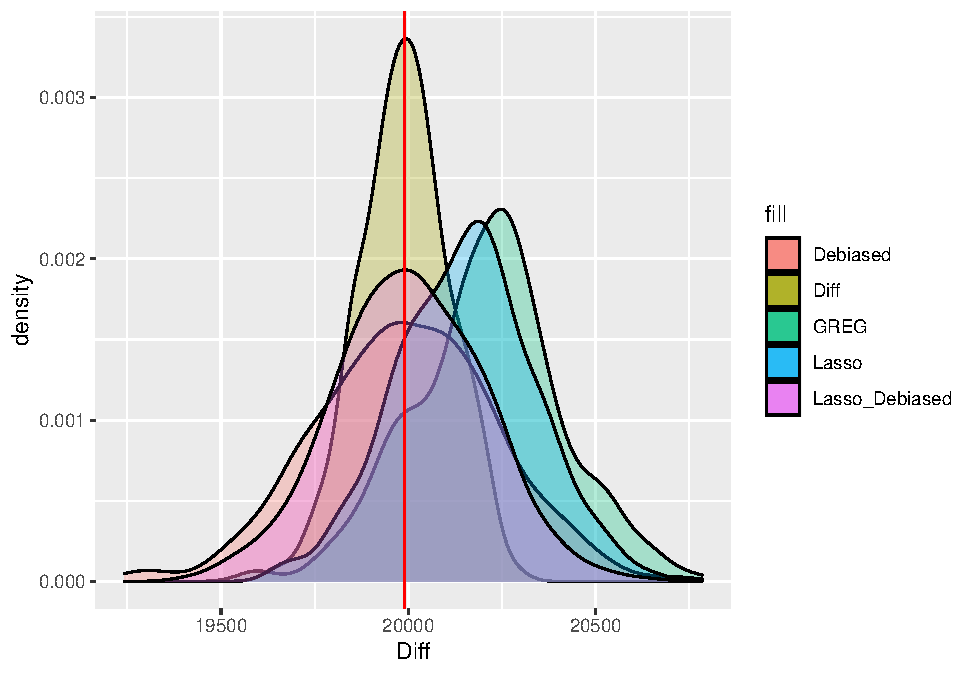
\includegraphics{sim/sim_092922_files/figure-latex/unnamed-chunk-3-1.pdf}


\begin{comment}
When does the GREG estimator have a large bias?
\begin{itemize}
    \item When the sample size is small
    \item When the variable of interest cannot be fit with a linear model
    \begin{itemize}
        \item We use a non-linear model.
    \end{itemize}
    \item When the sampling scheme is informative
\end{itemize}    
\end{comment}

\bibliographystyle{chicago}
\bibliography{ref}

\end{document}
